
%% IAENG_pub.tex 2010/08/30
%% It is based on the bare_jrnl.tex V1.3 2007/01/11 by Michael Shell
%% see http://www.michaelshell.org/
%% for current contact information.
%%
%% This is a skeleton file demonstrating the use of IAENGtran.cls
%% (requires IAENGtran.cls version 1.7 or later) with an IAENG journal/conference paper.
%%
%% Support sites:
%% http://www.michaelshell.org/tex
%% http://www.ctan.org/tex-archive/macros/latex/contrib/IEEEtran/

% *** Authors should verify (and, if needed, correct) their LaTeX system  ***
% *** with the testflow diagnostic prior to trusting their LaTeX platform ***
% *** with production work. IAENG's font choices can trigger bugs that do  ***
% *** not appear when using other class files.                            ***
% The testflow support page is at:
% http://www.michaelshell.org/tex/testflow/


%%*************************************************************************
%% Legal Notice:
%% This code is offered as-is without any warranty either expressed or
%% implied; without even the implied warranty of MERCHANTABILITY or
%% FITNESS FOR A PARTICULAR PURPOSE!
%% User assumes all risk.
%% In no event shall IAENG or any contributor to this code be liable for
%% any damages or losses, including, but not limited to, incidental,
%% consequential, or any other damages, resulting from the use or misuse
%% of any information contained here.
%%
%% All comments are the opinions of their respective authors and are not
%% necessarily endorsed by the IAENG.
%%
%% This work is distributed under the LaTeX Project Public License (LPPL)
%% ( http://www.latex-project.org/ ) version 1.3, and may be freely used,
%% distributed and modified. A copy of the LPPL, version 1.3, is included
%% in the base LaTeX documentation of all distributions of LaTeX released
%% 2003/12/01 or later.
%% Retain all contribution notices and credits.
%% ** Modified files should be clearly indicated as such, including  **
%% ** renaming them and changing author support contact information. **
%%
%%*************************************************************************

% Note that the a4paper option is mainly intended so that authors in
% countries using A4 can easily print to A4 and see how their papers will
% look in print - the typesetting of the document will not typically be
% affected with changes in paper size (but the bottom and side margins will).
% Use the testflow package mentioned above to verify correct handling of
% both paper sizes by the user's LaTeX system.
%
% Also note that the "draftcls" or "draftclsnofoot", not "draft", option
% should be used if it is desired that the figures are to be displayed in
% draft mode.
%
\documentclass[journal]{IAENGtran}
%
% If IAENGtran.cls has not been installed into the LaTeX system files,
% manually specify the path to it like:
% \documentclass[journal]{../sty/IAENGtran}





% Some very useful LaTeX packages include:
% (uncomment the ones you want to load)


% *** MISC UTILITY PACKAGES ***
%
%\usepackage{ifpdf}
% Heiko Oberdiek's ifpdf.sty is very useful if you need conditional
% compilation based on whether the output is pdf or dvi.
% usage:
% \ifpdf
%   % pdf code
% \else
%   % dvi code
% \fi
% The latest version of ifpdf.sty can be obtained from:
% http://www.ctan.org/tex-archive/macros/latex/contrib/oberdiek/
% Also, note that IAENGtran.cls V1.7 and later provides a builtin
% \ifCLASSINFOpdf conditional that works the same way.
% When switching from latex to pdflatex and vice-versa, the compiler may
% have to be run twice to clear warning/error messages.






% *** CITATION PACKAGES ***
%
%\usepackage{cite}
% cite.sty was written by Donald Arseneau
% V1.6 and later of IAENGtran pre-defines the format of the cite.sty package
% \cite{} output to follow that of IAENG. Loading the cite package will
% result in citation numbers being automatically sorted and properly
% "compressed/ranged". e.g., [1], [9], [2], [7], [5], [6] without using
% cite.sty will become [1], [2], [5]--[7], [9] using cite.sty. cite.sty's
% \cite will automatically add leading space, if needed. Use cite.sty's
% noadjust option (cite.sty V3.8 and later) if you want to turn this off.
% cite.sty is already installed on most LaTeX systems. Be sure and use
% version 4.0 (2003-05-27) and later if using hyperref.sty. cite.sty does
% not currently provide for hyperlinked citations.
% The latest version can be obtained at:
% http://www.ctan.org/tex-archive/macros/latex/contrib/cite/
% The documentation is contained in the cite.sty file itself.






% *** GRAPHICS RELATED PACKAGES ***
%
\ifCLASSINFOpdf
   \usepackage[pdftex]{graphicx}
  % declare the path(s) where your graphic files are
  % \graphicspath{{../pdf/}{../jpeg/}}
  % and their extensions so you won't have to specify these with
  % every instance of \includegraphics
   \DeclareGraphicsExtensions{.pdf,.jpeg,.png}
\else
  % or other class option (dvipsone, dvipdf, if not using dvips). graphicx
  % will default to the driver specified in the system graphics.cfg if no
  % driver is specified.
   \usepackage[dvips]{graphicx}
  % declare the path(s) where your graphic files are
  % \graphicspath{{../eps/}}
  % and their extensions so you won't have to specify these with
  % every instance of \includegraphics
   \DeclareGraphicsExtensions{.eps}
\fi
% graphicx was written by David Carlisle and Sebastian Rahtz. It is
% required if you want graphics, photos, etc. graphicx.sty is already
% installed on most LaTeX systems. The latest version and documentation can
% be obtained at:
% http://www.ctan.org/tex-archive/macros/latex/required/graphics/
% Another good source of documentation is "Using Imported Graphics in
% LaTeX2e" by Keith Reckdahl which can be found as epslatex.ps or
% epslatex.pdf at: http://www.ctan.org/tex-archive/info/
%
% latex, and pdflatex in dvi mode, support graphics in encapsulated
% postscript (.eps) format. pdflatex in pdf mode supports graphics
% in .pdf, .jpeg, .png and .mps (metapost) formats. Users should ensure
% that all non-photo figures use a vector format (.eps, .pdf, .mps) and
% not a bitmapped formats (.jpeg, .png). IAENG frowns on bitmapped formats
% which can result in "jaggedy"/blurry rendering of lines and letters as
% well as large increases in file sizes.
%
% You can find documentation about the pdfTeX application at:
% http://www.tug.org/applications/pdftex





% *** MATH PACKAGES ***
%
%\usepackage[cmex10]{amsmath}
% A popular package from the American Mathematical Society that provides
% many useful and powerful commands for dealing with mathematics. If using
% it, be sure to load this package with the cmex10 option to ensure that
% only type 1 fonts will utilized at all point sizes. Without this option,
% it is possible that some math symbols, particularly those within
% footnotes, will be rendered in bitmap form which will result in a
% document that can not be IAENG compliant!
%
% Also, note that the amsmath package sets \interdisplaylinepenalty to 10000
% thus preventing page breaks from occurring within multiline equations. Use:
%\interdisplaylinepenalty=2500
% after loading amsmath to restore such page breaks as IAENGtran.cls normally
% does. amsmath.sty is already installed on most LaTeX systems. The latest
% version and documentation can be obtained at:
% http://www.ctan.org/tex-archive/macros/latex/required/amslatex/math/





% *** SPECIALIZED LIST PACKAGES ***
%
%\usepackage{algorithmic}
% algorithmic.sty was written by Peter Williams and Rogerio Brito.
% This package provides an algorithmic environment for describing algorithms.
% You can use the algorithmic environment in-text or within a figure
% environment to provide for a floating algorithm. Do NOT use the algorithm
% floating environment provided by algorithm.sty (by the same authors) or
% algorithm2e.sty (by Christophe Fiorio) as IAENG does not use dedicated
% algorithm float types and packages that provide these will not provide
% correct IAENG style captions. The latest version and documentation of
% algorithmic.sty can be obtained at:
% http://www.ctan.org/tex-archive/macros/latex/contrib/algorithms/
% There is also a support site at:
% http://algorithms.berlios.de/index.html
% Also of interest may be the (relatively newer and more customizable)
% algorithmicx.sty package by Szasz Janos:
% http://www.ctan.org/tex-archive/macros/latex/contrib/algorithmicx/




% *** ALIGNMENT PACKAGES ***
%
%\usepackage{array}
% Frank Mittelbach's and David Carlisle's array.sty patches and improves
% the standard LaTeX2e array and tabular environments to provide better
% appearance and additional user controls. As the default LaTeX2e table
% generation code is lacking to the point of almost being broken with
% respect to the quality of the end results, all users are strongly
% advised to use an enhanced (at the very least that provided by array.sty)
% set of table tools. array.sty is already installed on most systems. The
% latest version and documentation can be obtained at:
% http://www.ctan.org/tex-archive/macros/latex/required/tools/


%\usepackage{mdwmath}
%\usepackage{mdwtab}
% Also highly recommended is Mark Wooding's extremely powerful MDW tools,
% especially mdwmath.sty and mdwtab.sty which are used to format equations
% and tables, respectively. The MDWtools set is already installed on most
% LaTeX systems. The lastest version and documentation is available at:
% http://www.ctan.org/tex-archive/macros/latex/contrib/mdwtools/


% IAENGtran contains the IAENGeqnarray family of commands that can be used to
% generate multiline equations as well as matrices, tables, etc., of high
% quality.


%\usepackage{eqparbox}
% Also of notable interest is Scott Pakin's eqparbox package for creating
% (automatically sized) equal width boxes - aka "natural width parboxes".
% Available at:
% http://www.ctan.org/tex-archive/macros/latex/contrib/eqparbox/





% *** SUBFIGURE PACKAGES ***
%\usepackage[tight,footnotesize]{subfigure}
% subfigure.sty was written by Steven Douglas Cochran. This package makes it
% easy to put subfigures in your figures. e.g., "Figure 1a and 1b". For IAENG
% work, it is a good idea to load it with the tight package option to reduce
% the amount of white space around the subfigures. subfigure.sty is already
% installed on most LaTeX systems. The latest version and documentation can
% be obtained at:
% http://www.ctan.org/tex-archive/obsolete/macros/latex/contrib/subfigure/
% subfigure.sty has been superceeded by subfig.sty.



%\usepackage[caption=false]{caption}
%\usepackage[font=footnotesize]{subfig}
% subfig.sty, also written by Steven Douglas Cochran, is the modern
% replacement for subfigure.sty. However, subfig.sty requires and
% automatically loads Axel Sommerfeldt's caption.sty which will override
% IAENGtran.cls handling of captions and this will result in nonIAENG style
% figure/table captions. To prevent this problem, be sure and preload
% caption.sty with its "caption=false" package option. This is will preserve
% IAENGtran.cls handing of captions. Version 1.3 (2005/06/28) and later
% (recommended due to many improvements over 1.2) of subfig.sty supports
% the caption=false option directly:
%\usepackage[caption=false,font=footnotesize]{subfig}
%
% The latest version and documentation can be obtained at:
% http://www.ctan.org/tex-archive/macros/latex/contrib/subfig/
% The latest version and documentation of caption.sty can be obtained at:
% http://www.ctan.org/tex-archive/macros/latex/contrib/caption/




% *** FLOAT PACKAGES ***
%
%\usepackage{fixltx2e}
% fixltx2e, the successor to the earlier fix2col.sty, was written by
% Frank Mittelbach and David Carlisle. This package corrects a few problems
% in the LaTeX2e kernel, the most notable of which is that in current
% LaTeX2e releases, the ordering of single and double column floats is not
% guaranteed to be preserved. Thus, an unpatched LaTeX2e can allow a
% single column figure to be placed prior to an earlier double column
% figure. The latest version and documentation can be found at:
% http://www.ctan.org/tex-archive/macros/latex/base/



%\usepackage{stfloats}
% stfloats.sty was written by Sigitas Tolusis. This package gives LaTeX2e
% the ability to do double column floats at the bottom of the page as well
% as the top. (e.g., "\begin{figure*}[!b]" is not normally possible in
% LaTeX2e). It also provides a command:
%\fnbelowfloat
% to enable the placement of footnotes below bottom floats (the standard
% LaTeX2e kernel puts them above bottom floats). This is an invasive package
% which rewrites many portions of the LaTeX2e float routines. It may not work
% with other packages that modify the LaTeX2e float routines. The latest
% version and documentation can be obtained at:
% http://www.ctan.org/tex-archive/macros/latex/contrib/sttools/
% Documentation is contained in the stfloats.sty comments as well as in the
% presfull.pdf file. Do not use the stfloats baselinefloat ability as IAENG
% does not allow \baselineskip to stretch. Authors submitting work to the
% IAENG should note that IAENG rarely uses double column equations and
% that authors should try to avoid such use. Do not be tempted to use the
% cuted.sty or midfloat.sty packages (also by Sigitas Tolusis) as IAENG does
% not format its papers in such ways.


%\ifCLASSOPTIONcaptionsoff
%  \usepackage[nomarkers]{endfloat}
% \let\MYoriglatexcaption\caption
% \renewcommand{\caption}[2][\relax]{\MYoriglatexcaption[#2]{#2}}
%\fi
% endfloat.sty was written by James Darrell McCauley and Jeff Goldberg.
% This package may be useful when used in conjunction with IAENGtran.cls'
% captionsoff option. Some IAENG journals/societies require that submissions
% have lists of figures/tables at the end of the paper and that
% figures/tables without any captions are placed on a page by themselves at
% the end of the document. If needed, the draftcls IAENGtran class option or
% \CLASSINPUTbaselinestretch interface can be used to increase the line
% spacing as well. Be sure and use the nomarkers option of endfloat to
% prevent endfloat from "marking" where the figures would have been placed
% in the text. The two hack lines of code above are a slight modification of
% that suggested by in the endfloat docs (section 8.3.1) to ensure that
% the full captions always appear in the list of figures/tables - even if
% the user used the short optional argument of \caption[]{}.
% IAENG papers do not typically make use of \caption[]'s optional argument,
% so this should not be an issue. A similar trick can be used to disable
% captions of packages such as subfig.sty that lack options to turn off
% the subcaptions:
% For subfig.sty:
% \let\MYorigsubfloat\subfloat
% \renewcommand{\subfloat}[2][\relax]{\MYorigsubfloat[]{#2}}
% For subfigure.sty:
% \let\MYorigsubfigure\subfigure
% \renewcommand{\subfigure}[2][\relax]{\MYorigsubfigure[]{#2}}
% However, the above trick will not work if both optional arguments of
% the \subfloat/subfig command are used. Furthermore, there needs to be a
% description of each subfigure *somewhere* and endfloat does not add
% subfigure captions to its list of figures. Thus, the best approach is to
% avoid the use of subfigure captions (many IAENG journals avoid them anyway)
% and instead reference/explain all the subfigures within the main caption.
% The latest version of endfloat.sty and its documentation can obtained at:
% http://www.ctan.org/tex-archive/macros/latex/contrib/endfloat/
%
% The IAENGtran \ifCLASSOPTIONcaptionsoff conditional can also be used
% later in the document, say, to conditionally put the References on a
% page by themselves.





% *** PDF, URL AND HYPERLINK PACKAGES ***
%
%\usepackage{url}
% url.sty was written by Donald Arseneau. It provides better support for
% handling and breaking URLs. url.sty is already installed on most LaTeX
% systems. The latest version can be obtained at:
% http://www.ctan.org/tex-archive/macros/latex/contrib/misc/
% Read the url.sty source comments for usage information. Basically,
% \url{my_url_here}.





% *** Do not adjust lengths that control margins, column widths, etc. ***
% *** Do not use packages that alter fonts (such as pslatex).         ***
% There should be no need to do such things with IAENGtran.cls V1.6 and later.
% (Unless specifically asked to do so by the journal or conference you plan
% to submit to, of course. )


% correct bad hyphenation here
% \hyphenation{op-tical net-works semi-conduc-tor}

\newcommand{\secref}[1]{Section \ref{#1}}
\newcommand{\figref}[1]{Fig. \ref{#1}}
\newcommand{\tabref}[1]{Table \ref{#1}}

\newcommand{\publicationTitle}{An Approach for Test Case Generation from a Static Call Graph for Object-Oriented Programming}


\usepackage{adjustbox}
\begin{document}
%
% paper title
% can use linebreaks \\ within to get better formatting as desired
\title{{\publicationTitle}}
%
%
% author names and IAENG memberships
% note positions of commas and nonbreaking spaces ( ~ ) LaTeX will not break
% a structure at a ~ so this keeps an author's name from being broken across
% two lines.
% use \thanks{} to gain access to the first footnote area
% a separate \thanks must be used for each paragraph as LaTeX2e's \thanks
% was not built to handle multiple paragraphs
%

\author{Sitdhibong~Laokok and
        Taratip~Suwannasart % <-this % stops a space
\thanks{S. Laokok and T. Suwannasart are with the Department of Computer Engineering,
        Faculty of Engineering, Chulalongkorn University, Bangkok Thailand.}}% <-this % stops a space


% note the % following the last \IAENGmembership and also \thanks -
% these prevent an unwanted space from occurring between the last author name
% and the end of the author line. i.e., if you had this:
%
% \author{....lastname \thanks{...} \thanks{...} }
%                     ^------------^------------^----Do not want these spaces!
%
% a space would be appended to the last name and could cause every name on that
% line to be shifted left slightly. This is one of those "LaTeX things". For
% instance, "\textbf{A} \textbf{B}" will typeset as "A B" not "AB". To get
% "AB" then you have to do: "\textbf{A}\textbf{B}"
% \thanks is no different in this regard, so shield the last } of each \thanks
% that ends a line with a % and do not let a space in before the next \thanks.
% Spaces after \IAENGmembership other than the last one are OK (and needed) as
% you are supposed to have spaces between the names. For what it is worth,
% this is a minor point as most people would not even notice if the said evil
% space somehow managed to creep in.



% The paper headers
%\markboth{}%
%{Shell \MakeLowercase{\textit{et al.}}:}
% The only time the second header will appear is for the odd numbered pages
% after the title page when using the twoside option.
%
% *** Note that you probably will NOT want to include the author's ***
% *** name in the headers of peer review papers.                   ***
% You can use \ifCLASSOPTIONpeerreview for conditional compilation here if
% you desire.




% If you want to put a publisher's ID mark on the page you can do it like
% this:
%\IAENGpubid{0000--0000/00\$00.00~\copyright~2007 IAENG}
% Remember, if you use this you must call \IAENGpubidadjcol in the second
% column for its text to clear the IAENGpubid mark.



% use for special paper notices
%\IAENGspecialpapernotice{(Invited Paper)}




% make the title area
\maketitle

\pagestyle{empty}
\thispagestyle{empty}


\begin{abstract}
%\boldmath
    In software development, a software testing is a mandatory process
    to indicate the quality level of the software and to verify that
    all components have been working properly. For integration testing,
    it is a testing process used to verify the efficiency and to uncover
    errors occurring between class interfaces. This error indicating method 
    may be expensive due to the reason that each class might have numbers 
    of interfaces that need to be considered in source code. 
    This paper aims at proposing an approach to generate test cases 
    in order to cover all class interfaces, including of branch coverage, 
    by collecting data from source code and generating a static call graph, 
    which will represent all class interfaces found in source code. 
    Moreover, our can gather appropriate data to support 
    the generated test cases. 
\end{abstract}
% IAENGtran.cls defaults to using nonbold math in the Abstract.
% This preserves the distinction between vectors and scalars. However,
% if the journal you are submitting to favors bold math in the abstract,
% then you can use LaTeX's standard command \boldmath at the very start
% of the abstract to achieve this. Many IAENG journals frown on math
% in the abstract anyway.

% Note that keywords are not normally used for peerreview papers.
\begin{IAENGkeywords}
    Control Flow Graph, Static Call Graph, Test Case Generation
\end{IAENGkeywords}

% For peer review papers, you can put extra information on the cover
% page as needed:
% \ifCLASSOPTIONpeerreview
% \begin{center} \bfseries EDICS Category: 3-BBND \end{center}
% \fi
%
% For peerreview papers, this IAENGtran command inserts a page break and
% creates the second title. It will be ignored for other modes.
\IAENGpeerreviewmaketitle

\section{Introduction}
% The very first letter is a 2 line initial drop letter followed
% by the rest of the first word in caps.
%
% form to use if the first word consists of a single letter:
% \IAENGPARstart{A}{demo} file is ....
%
% form to use if you need the single drop letter followed by
% normal text (unknown if ever used by IAENG):
% \IAENGPARstart{A}{}demo file is ....
%
% Some journals put the first two words in caps:
% \IAENGPARstart{T}{his demo} file is ....
%
% Here we have the typical use of a "T" for an initial drop letter
% and "HIS" in caps to complete the first word.
\IAENGPARstart{S}{oftware} testing is an important process 
to indicate the confidence level of Software Under Testing (SUT) 
by verifying conformance to Software Requirements Specification (SRS) 
and uncovering errors that still remain in source code \cite{Jorgensen2013}.
In order to perform a software testing, a software tester is required 
to read between the lines of code to generate a set of test case, test suite, 
and test data. This is to cover all interested software components. 
The software tester should have numbers of approaches to determine 
coverage criteria that are to be achieved.

While the test case generation is performed, the software tester has 
to read between the lines of code in order to understand 
the source code structure of SUT. There are several approaches 
that a software tester can use to represent the source code structure. 
Normally, Control Flow Graph (CFG) is widely used, as it makes source code 
more understandable even when the software tester is not familiar with 
the language used by developers. In addition, the software tester will 
also have to be able to derive test cases from CFG by picking up 
interested paths to be the test paths. Then, the software tester has to 
generate test data by considering the test path in order to assure 
that each test path is working well along with the generated test cases. 
Besides, the software tester has to set the goal before selecting the 
test paths. In path-oriented, the software tester must generate test cases 
to cover all branches in the source code structure (Branch-coverage) or 
to cover all predicate nodes \cite{Luanghirun2016}.

For object-oriented programming, software is composed of classes 
that work together by sending signal to one another. The approach to 
the test case generation cannot focus on only an individual class, 
but it has to focus on the connection between them during 
the integration testing process, as errors can occur anytime 
when objects are connected.

During the integration testing process, the test case should cover all 
components that are found in source code in order to find errors occurring 
in each path that is placed between classes. Test case generation 
to cover all the existing paths of the source code structure 
is an expensive process, because the software tester has to seek 
for all paths one by one. The Static Call Graph (SCG), which is a graph 
that represents the connections between classes, will assist the 
software tester to generate the test case in order to validate 
all connected paths by gathering data from source code.

In this paper, we aim to propose test cases, which is generated 
from a call graph retrieved from source code, in order to 
represent all of the connections between objects. Moreover, 
we also propose test data generation, which complies with the test 
paths that the software tester has picked up.

The rest of the paper is organized as follows. Section II discusses 
existing works done based on the path-oriented method. 
Section III introduces the background of the program graph, SCG, CFG, 
and automated test case generation techniques. 
For Section IV presents the approach to test case generation 
and test data retrieved from SCG and CFG. Lastly, Section V 
concludes all the contents provided in this paper, altogether with future work.

%\hfill mds
%\hfill January 11, 2007


\section{Related Works}

Unit test is a testing process to locate errors in SUT by focusing 
only on the interested parts and eliminate interaction occurred 
between software components by creating a drive or stub 
\cite{Jorgensen2013}. In contrast, integration testing is a process 
to uncover errors that may occur even though all the components 
have been working properly together \cite{Jalote:1997:IAS:549018}; however, the test case 
for this process that has to cover all of the class interfaces 
is expensive, as there are a large number of interfaces between 
classes that must be considered by the software tester. 
V. Panthini and D. Prasad \cite{4425952} has proposed a generated test case 
based on a sequence diagram in order to identify interactions 
between objects. However, the sequence diagram may not reflect 
the current state of source code, due to the reason 
that source code might be changed to another appropriate development 
methodology or techniques. S. Z. Waheed and U. Qamar \cite{7339088} 
has proposed that the test case generation for the integration testing 
is based on the flow diagram data and selected DU 
paths that are used to be the test path.  However, software 
is a result of class communication and the test path 
must be as long as possible to traverse each component 
that used to work together.

According to the references given above, we found that there 
is not any approaches that generate a test case that can be traversed 
through selected test paths between objects which have been working 
together based on object-oriented development in order to cover 
all branch interfaces found in source code. In addition, 
we are confident that our proposal will come up with an appropriate 
data set for the future test case generations.


\section{Background}

\subsection{Program Graph}

Software has been developed with multiple purposes and made 
source code become more complicated. The designing diagram 
is used here to illustrate how source code works. However, 
source code is always changeable to fit with the language 
of developers. Therefore, a program graph is a graph 
that is used to represent the structure of source code and 
to reflect the current version of it.

\begin{figure}[ht!]
    \centering
    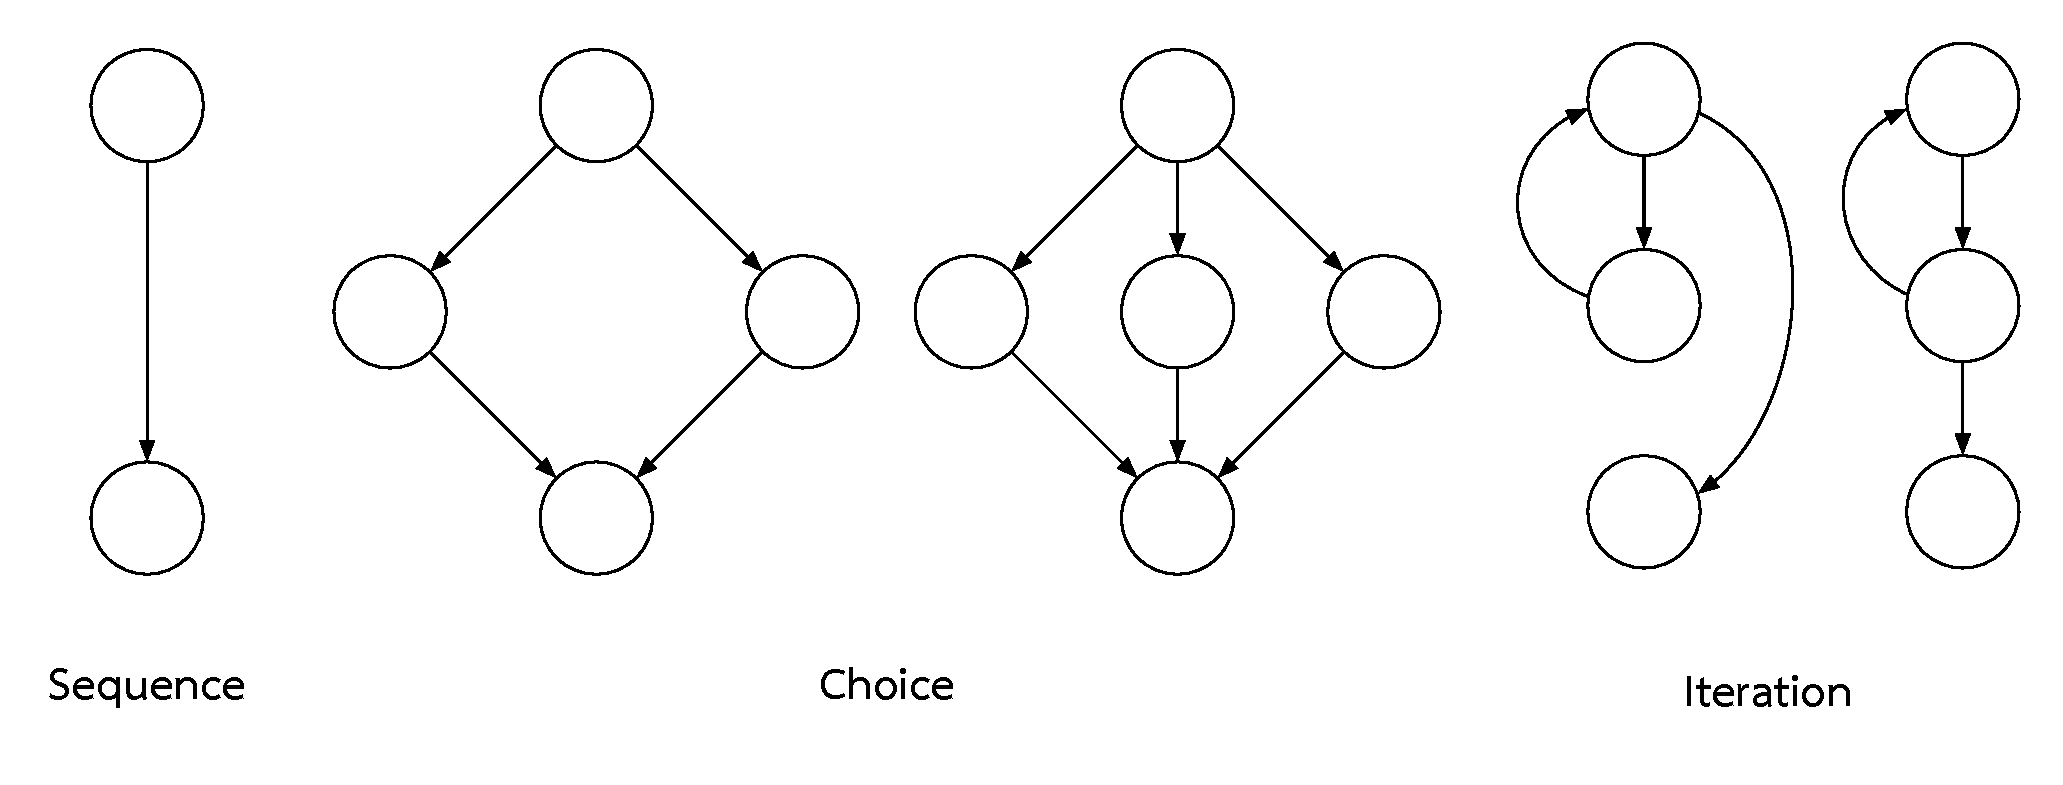
\includegraphics[width=0.9\linewidth]{figures/Primitive-Operation-Structure}
    \caption{The Primitive Operations of Structured Programming}
    \label{fig:primitiveoperations}
\end{figure}

\subsubsection{Control Flow Graph}
With difference purposes of software to be developed, 
there are several platforms and languages 
that software developer use for develop software. 
Therefore, it might be difficult for the software tester, 
as he or she may not be familiar with all of these differences. 
CFG is able to represent the structure of source code in 
the form of graph. CFG is Directed Acyclic Graph (DAG) 
that could represent the structure of source code and relationship 
between the lines of code with nodes and edges. It starts from 
the source node to sink node through the sequences of nodes, 
which are connected by edges. CFG with its primitive structure 
was defined by McCabe \cite{McCabe1976}  as shown in 
\figref{fig:primitiveoperations} The software tester should 
analyze CFG and select the test path, which traverses from 
the source node through nodes in the graph with a purpose 
to cover each branch and exercise all predicate nodes in the graph.


\subsubsection{Static Call Graph}
Software is composed of classes, which work together by calling 
their own methods or other methods from other classes. 
SCG, which is a Directed Multiple Graph, represents the relationships 
between classes in SUT, in which each node represents classes 
and edge represents calling of method. In general, there can be 
several outdegree in a single node. SCG is formed by collecting 
calling statements found in source code, in which the called method 
has been called from the calling method for the other classes. 
Only when SCG illustrates the current source code structure, 
the software tester will be able to analyze the interfaces 
between classes to generate a test case that will cover 
all the interfaces in SUT.

\begin{figure}[ht!]
    \centering
    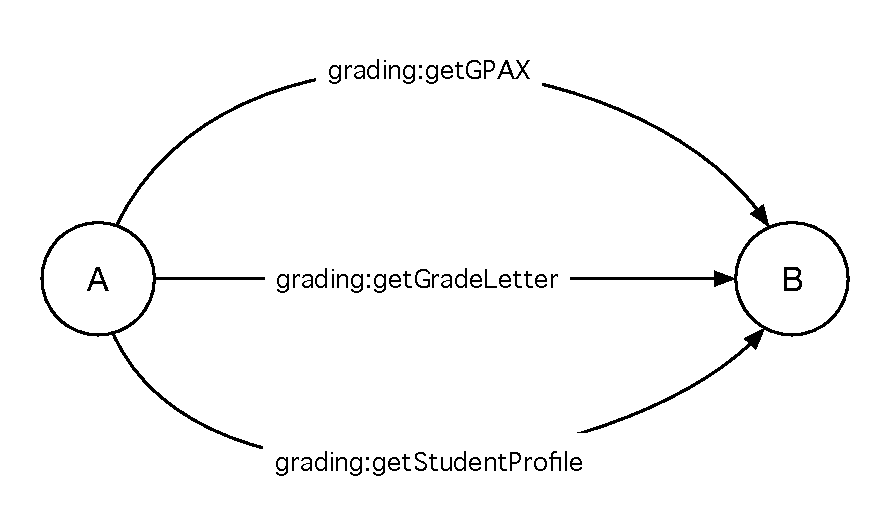
\includegraphics[width=0.9\linewidth]{figures/SCG-A-and-B}
    \caption{Static Call Graph of Class A and Class B}
    \label{fig:scgAandB}
\end{figure}

In \figref{fig:scgAandB} shows an example of SCG that represents 
the relationships between class $A$ and class $B$, Where class $A$ has 
3 calling statements in calling method, grading, that calls 
to called method $getGPAX$, $getGradeLetter$, and $getStudentProfile$ 
in class $B$. Calling and called method are separated with “$:$” 
and used for label the edge between class $A$ and $B$ 
such as “$grading:getGPAX$”. This relationship should be formed into 
$G = (V, E, l, p)$, where $G$ is a Multiple Call Graph, 
$V$ is a set of node, $E$ is a set of edge, $l$ is a set of label, 
$p$ is a function that maps each edge in $E$ to label in $l$. 
For this pair of nodes, $A$ is the head node and $B$ is the tail node 
\cite{Bang-Jensen:2008:DTA:1523254}.


\section{Proposed Approach}

\begin{figure}[ht!]
    \centering
    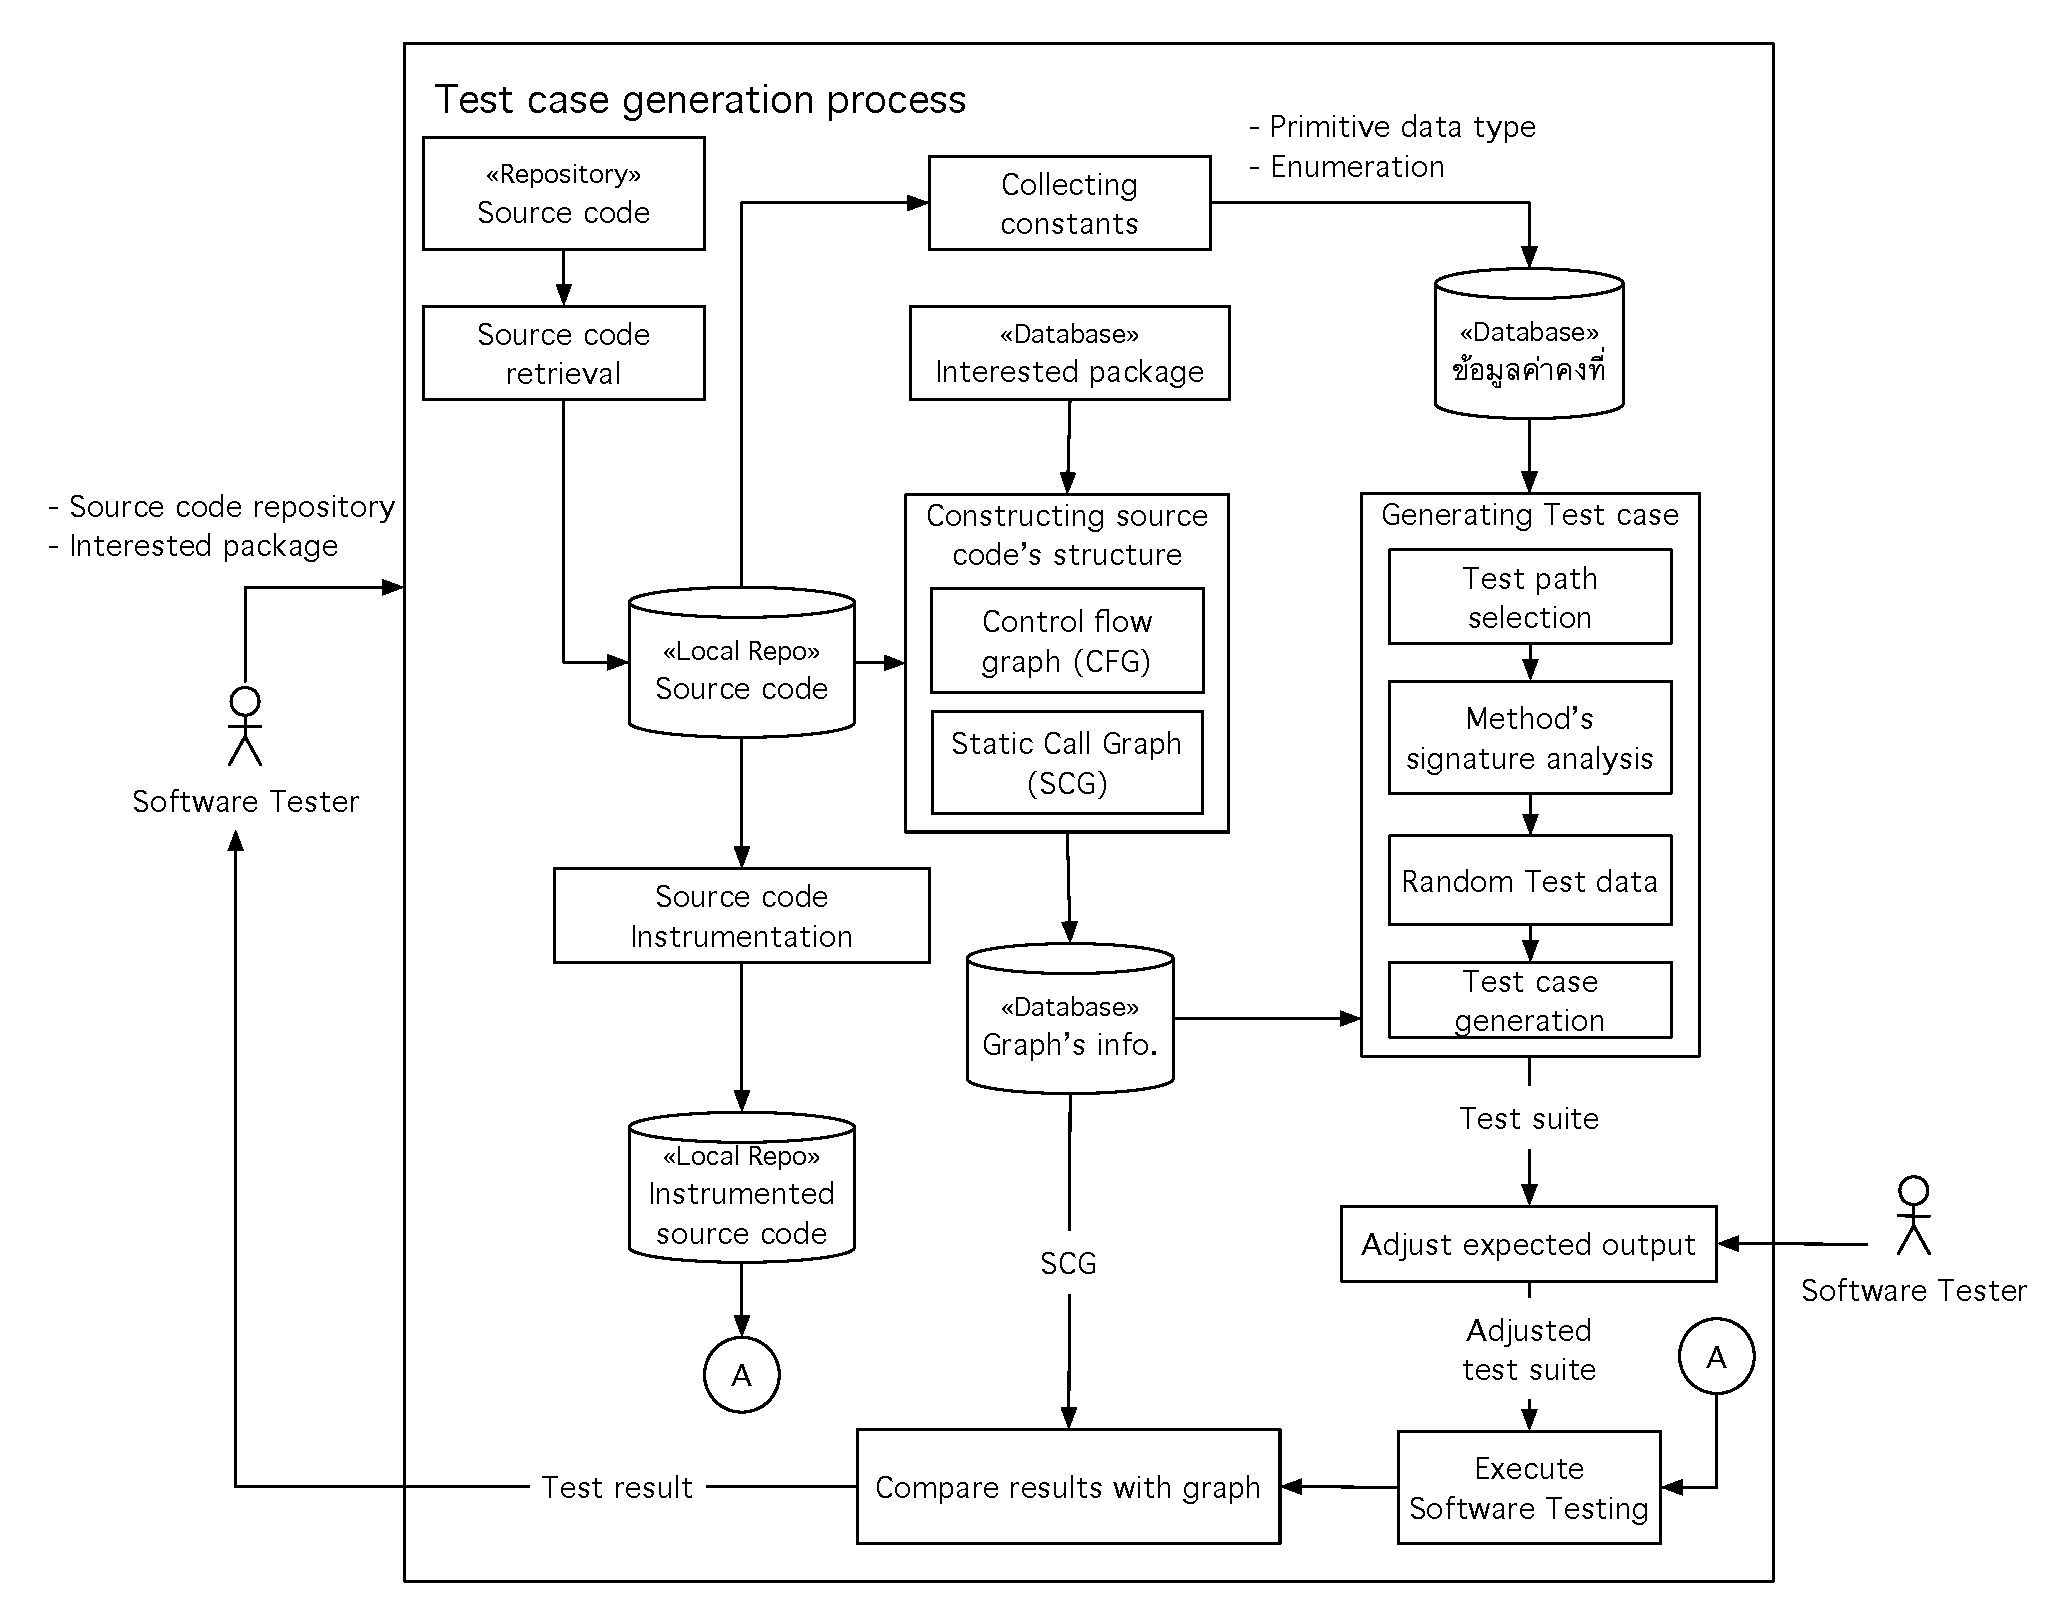
\includegraphics[width=\linewidth]{figures/Methodology}
    \caption{Methodology of Test Case Generation based on Static Data}
    \label{fig:methodology}
\end{figure}

In this section, we present our approach to test case generation 
based on SCG. A set of static data is gathered from source code 
and formed into SCG and CFG. We assure that the generated test case 
conforms to the selected test path. At the last step, we execute 
a test case that comes with instrumentation source code and display 
the result to the software tester. Each step of our approach 
is explained in \figref{fig:methodology}.

\subsection{Source Code Retrieval}

Source code repository is a place to store source code, 
determined by the software tester. At this step, we should 
retrieve source code to access the local repository.

\subsection{Constant Collection}

An object is composed of a primitive data set (booleans, 
numbers, and strings); however, an object which is composed 
of random data will normally fail to satisfy the conditions 
and is not possible to activate a specific path. Therefore, 
we need to find an appropriate value that possibly satisfies 
the criteria. We could say that a predefined primitive value 
in source code can be used to construct an object more potentially 
than the others \cite{McCabe1976}.

This process aims to analyze each class’s files stored within 
a certain package designated by the software tester to collect 
constant values. The collected primitive values should 
also lead to random satisfying values in order to cover 
the test paths \cite{McCabe1976}.

\subsection{Constructing Source Code’s Structure}

In order to form a satisfying condition for source code, 
the software tester has to understand its structure. Therefore, 
this process is to create graphs, CFG and SCG, which represent 
the structure of source code and eliminate infeasible paths. 
When the process ends, source code structure, the graphs, 
and all possible paths will be stored in the database. 
Soon after, the generated test case will retrieve data 
from the database to generate another test case that conforms 
to the selected test paths. For more detail, each step 
is clearly discussed as follows:

\subsubsection{Control Flow Graph Construction}

Source code within the assigned package is retrieved from 
the repository given by a software tester, and parses each statement 
into nodes is assigned. Then, it will assign a relationship 
of the source node and the other nodes, which work after 
the previous node, until nodes are all connected. Finally, we must 
keep all the feasible paths and source node to sync all of them in 
the form of graph in the database. For example, if $C_1$, $C_2$, 
and $C_3$ are classes within the interested package which contains 
method sets: \{$m_{11}$, $m_{12}$\}, \{$m_{21}$, $m_{22}$, $m_{23}$\}, 
and \{$m_{31}$, $m_{32}$\} respectively, CFG will be created 
from each method in a certain class.

From this process, we create CFG from source code to represent 
the source code structure. Furthermore, we also gather data 
from the steps of creating an object. These steps should be used 
as a reference in the test case generation process.

\subsubsection{Static Call Graph Construction}

This process collects the static data from source code 
for SCG construction. To perform this process, source code 
should be retrieved from the local repository. Then, calling statements 
that call to another class should be collected. A method that 
contains calling statements should be assigned to calling method, 
and a method is called in calling statement should be assigned 
to called method. To create SCG, in which each node represents classes 
in SUT and each edge represents the relationship between nodes. 
At the final phase, each edge will be labeled by the calling and 
called methods as shown in \figref{fig:relationship}

\begin{figure}[bh!]
\centering
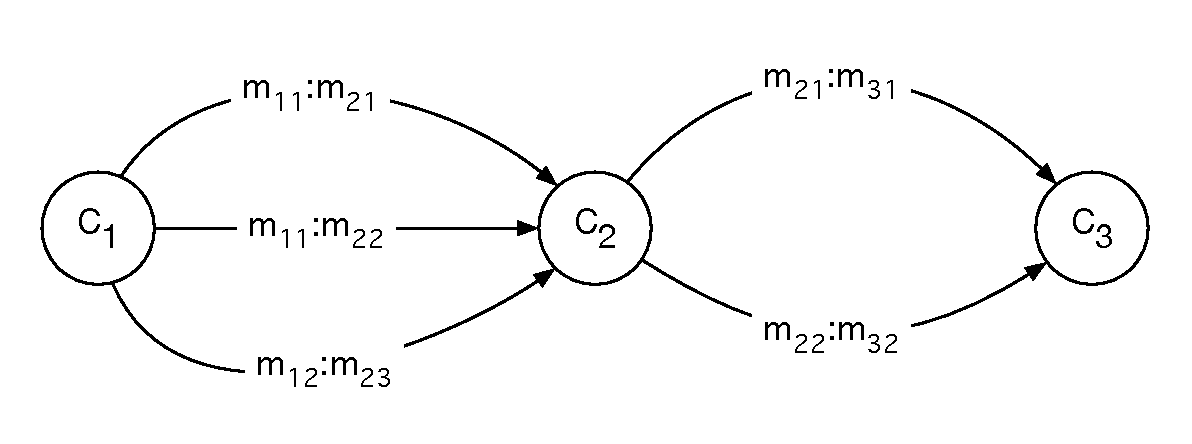
\includegraphics[width=\linewidth]{figures/Relationship-between-Classes}
\caption{Relationship between Classes $C_1$, $C_2$ and $C_3$}
\label{fig:relationship}
\end{figure}

\subsection{Source code instrumentation}

This process adds instrumentation message that displays 
a specific message when the test case has exercised through 
the lines. To make sure that the generated test cases have 
already covered all SCG’s branches (Branch coverage), at least once. 
Source code should be instrumented for monitoring if all branches 
are covered.

\subsubsection{Method Entry and Existence}
In statement instrumentation, the instrumentation message is 
added right after method declaration statement and before method 
ending or returning values. Message from this statement shows 
that test cases are able to exercise through methods 
between classes on test paths.

\subsubsection{Predicate Execution}
Selected test paths can be consisted of several predicate nodes. 
For this statement type, instrumentation message 
is added right after predicate statements.

\subsubsection{Calling Method}
Displaying message while methods between classed are invoked 
is the main goal of this approach. Instrumentation message 
is added right before and after finding these statements 
in order to display the message before and after invoking 
for method, respectively. For the message analysis, we analyze 
message from the entry method and explain the execution path 
for both invoking and invoke method.

After this process, instrumentation source code 
will be archived in the local repository.

\subsection{Test Case Generation}

In our approach, test cases are generated based on 
static data collected from source code. Previously, the constant 
and source code structures collected. This process analyze the data 
and generates test data and test cases in order to exercise 
each SCG’s branch at least one time. The process 
is shown as in \figref{fig:activitiesTC}

\subsubsection{Test Path Selection}
This process starts with retrieving all test paths of SCG and CFG 
structure formed in the database. Then, we should consider 
each pair of the SCG nodes. After that, the calling and called methods 
should be extracted from each edge label, one by one. For the next step, 
we should select CFG for calling node in order to analyze 
the test paths by finding the shortest path that contains calling nodes 
which represent to calling statements. This means that the first node pair 
of the test path is being selected. Next, the previous tail node 
is set to be the head node. Calling method is set to previously 
called method. Then, we repeat the test path selection steps in order to 
find all of the test paths. This is to achieve the branch coverage.

From SCG of class $C_1$, $C_2$, and $C_3$ as shown in \figref{fig:relationship}, 
we can get started from the nodes of $C_1$ and $C_2$ ($C_1$ is the head node, 
while $C_2$ is the tail node). After that, we have to extract the name of 
the calling and called methods from each of the edge labels. 
Therefore, $m_{11}$ and $m_{21}$ retrieved from the above edge should be 
calling and called methods respectively. After that, we have to find 
calling statements and called method, which are $m_{21}$, in $m_{11}$ from 
the structure of $m_{11}$ as shown in \figref{fig:cfgOfMethod}, given that node 16 is invoking node 
(invoking statement). Now, we have already generated test paths, $11-12-14-16-18-19$, 
from m11 to cover all the branches ($C_1$, $C_2$, $m_{11}:m_{12}$). Then, the head node 
will be changed from $C_1$ to $C_2$, and the invoking method will be changed 
from $m_{11}$ to $m_{21}$. When it comes to this final step, we need to repeat all 
over again if there are any edge labels that start with the invoking method. 
If there are no any edge labels with the invoking method left, we have to set 
the invoking method on another invoking method that is left on 
the previous head node.

\begin{figure}[ht!]
\centering
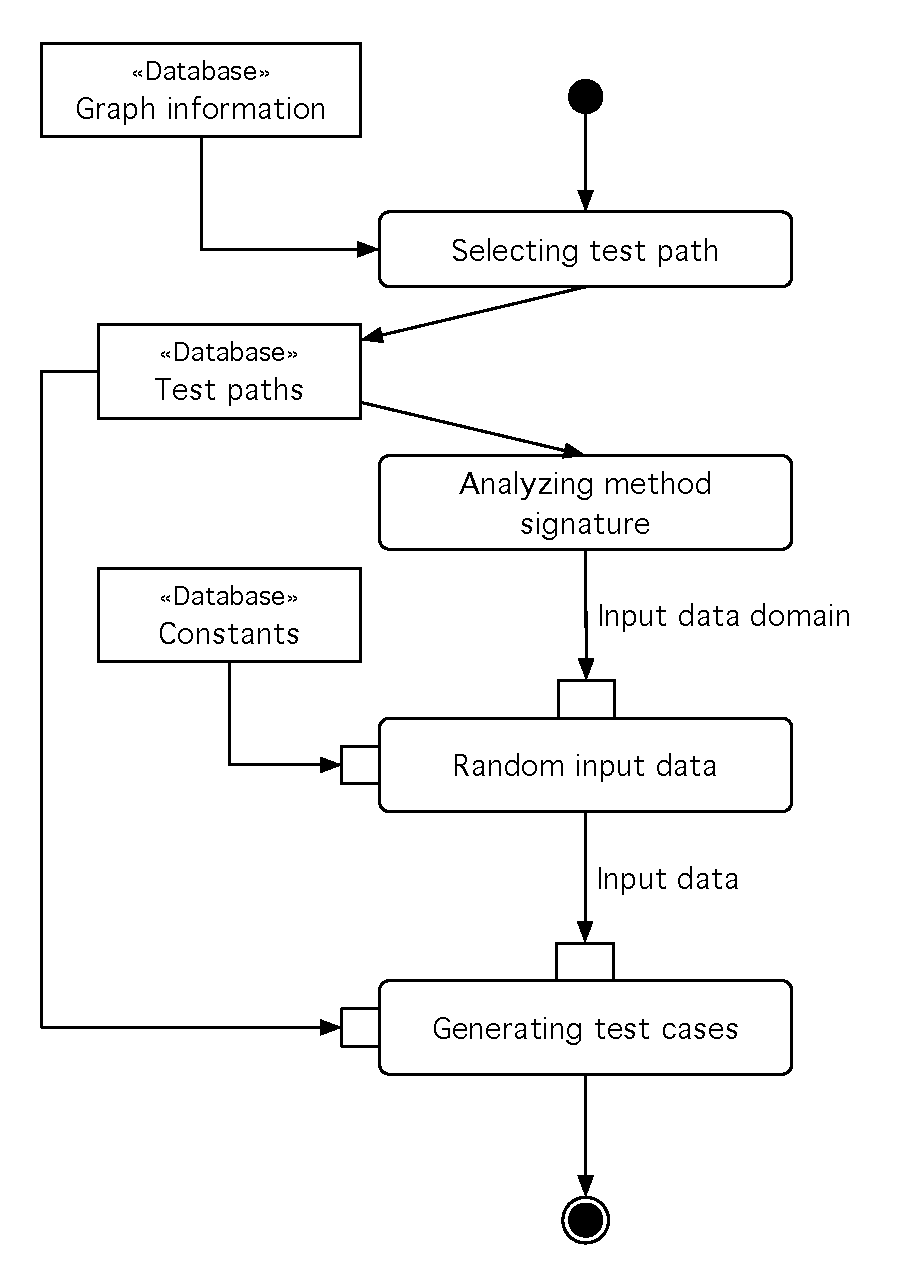
\includegraphics[width=0.7\linewidth]{figures/Activities}
\caption{Activities in Test Caset Generation Process}
\label{fig:activitiesTC}
\end{figure}

\begin{figure}[hb!]
\centering
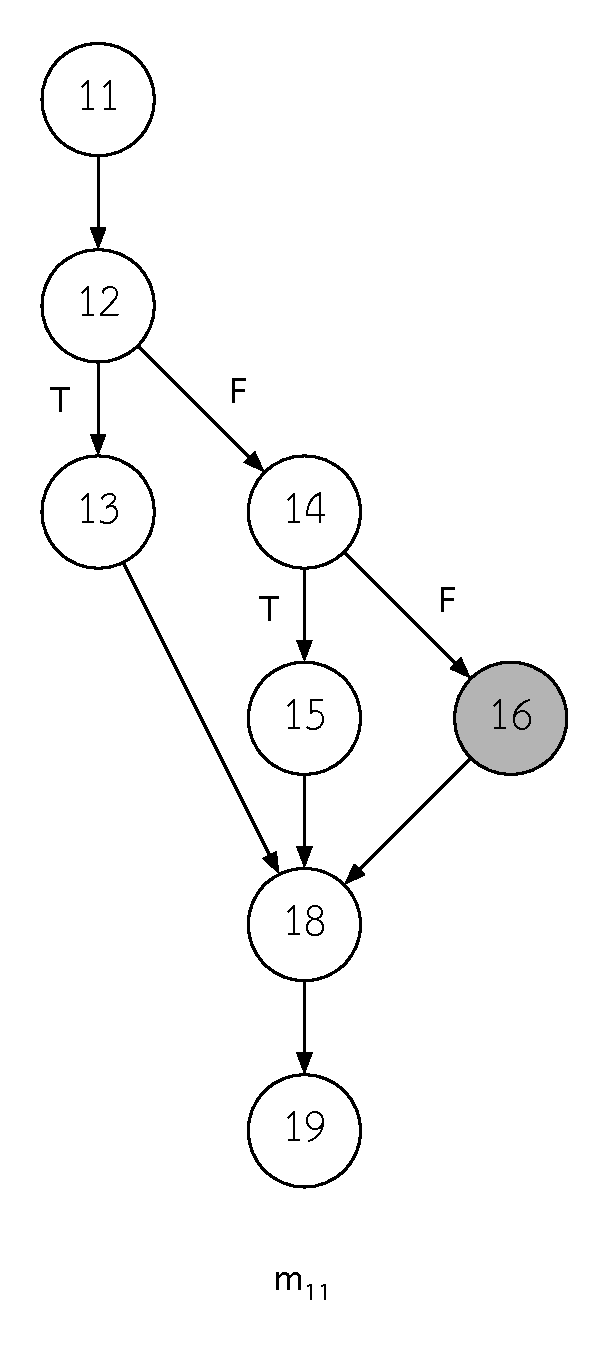
\includegraphics[width=0.4\linewidth]{figures/CFG-of-m11-in-c1}
\caption{Control Flow Graph of method $m_{11}$ of class $C_1$}
\label{fig:cfgOfMethod}
\end{figure}

According to the steps explained above, the test cases can be generated 
as shown in \tabref{tab:generatedTestCase}

\begin{table}[!t]
\renewcommand{\arraystretch}{1.3}
\caption{Generated Test Case from a Static Call Graph}
\label{tab:generatedTestCase}
\centering
\begin{tabular}{cl}
\hline
ID & Test Path \\ \hline
1  & ($C_1$, $C_2$, $m_{11}:m_{21}$) - ($C_2$, $C_3$, $m_{21}:m_{31}$) \\ \hline
2  & ($C_1$, $C_2$, $m_{11}:m_{22}$) - ($C_2$, $C_3$, $m_{22}:m_{32}$) \\ \hline
3  & ($C_1$, $C_2$, $m_{12}:m_{23}$) \\ \hline
\hline
\end{tabular}
\end{table}

For the test paths retrieved from SCG in \tabref{tab:generatedTestCase} we have to consider CFG 
of method $m_{11}$ within class $C_1$, method $m_{21}$ within class $C_2$, and finally 
method $m_{31}$ within class $C_3$. CFG shown in \figref{fig:callingStatement} is the CFG 
of $m_{11}$, $m_{21}$ and $m_{31}$ respectively. The generated test paths should be tuple of 
(($11$, $12$, $14$, $16$)$m_{11}$, ($10$, $11$, $17$)$m_{21}$, 
($10$, $11$, $12$, $14$, $18$, $19$)$m_{31}$, ($17$, $18$, $19$)$m_{21}$, ($16$, $18$, $19$)$m_{11}$). 
Finally, all test paths are sent to the signature analysis method for the next process.

\begin{figure}[ht!]
\centering
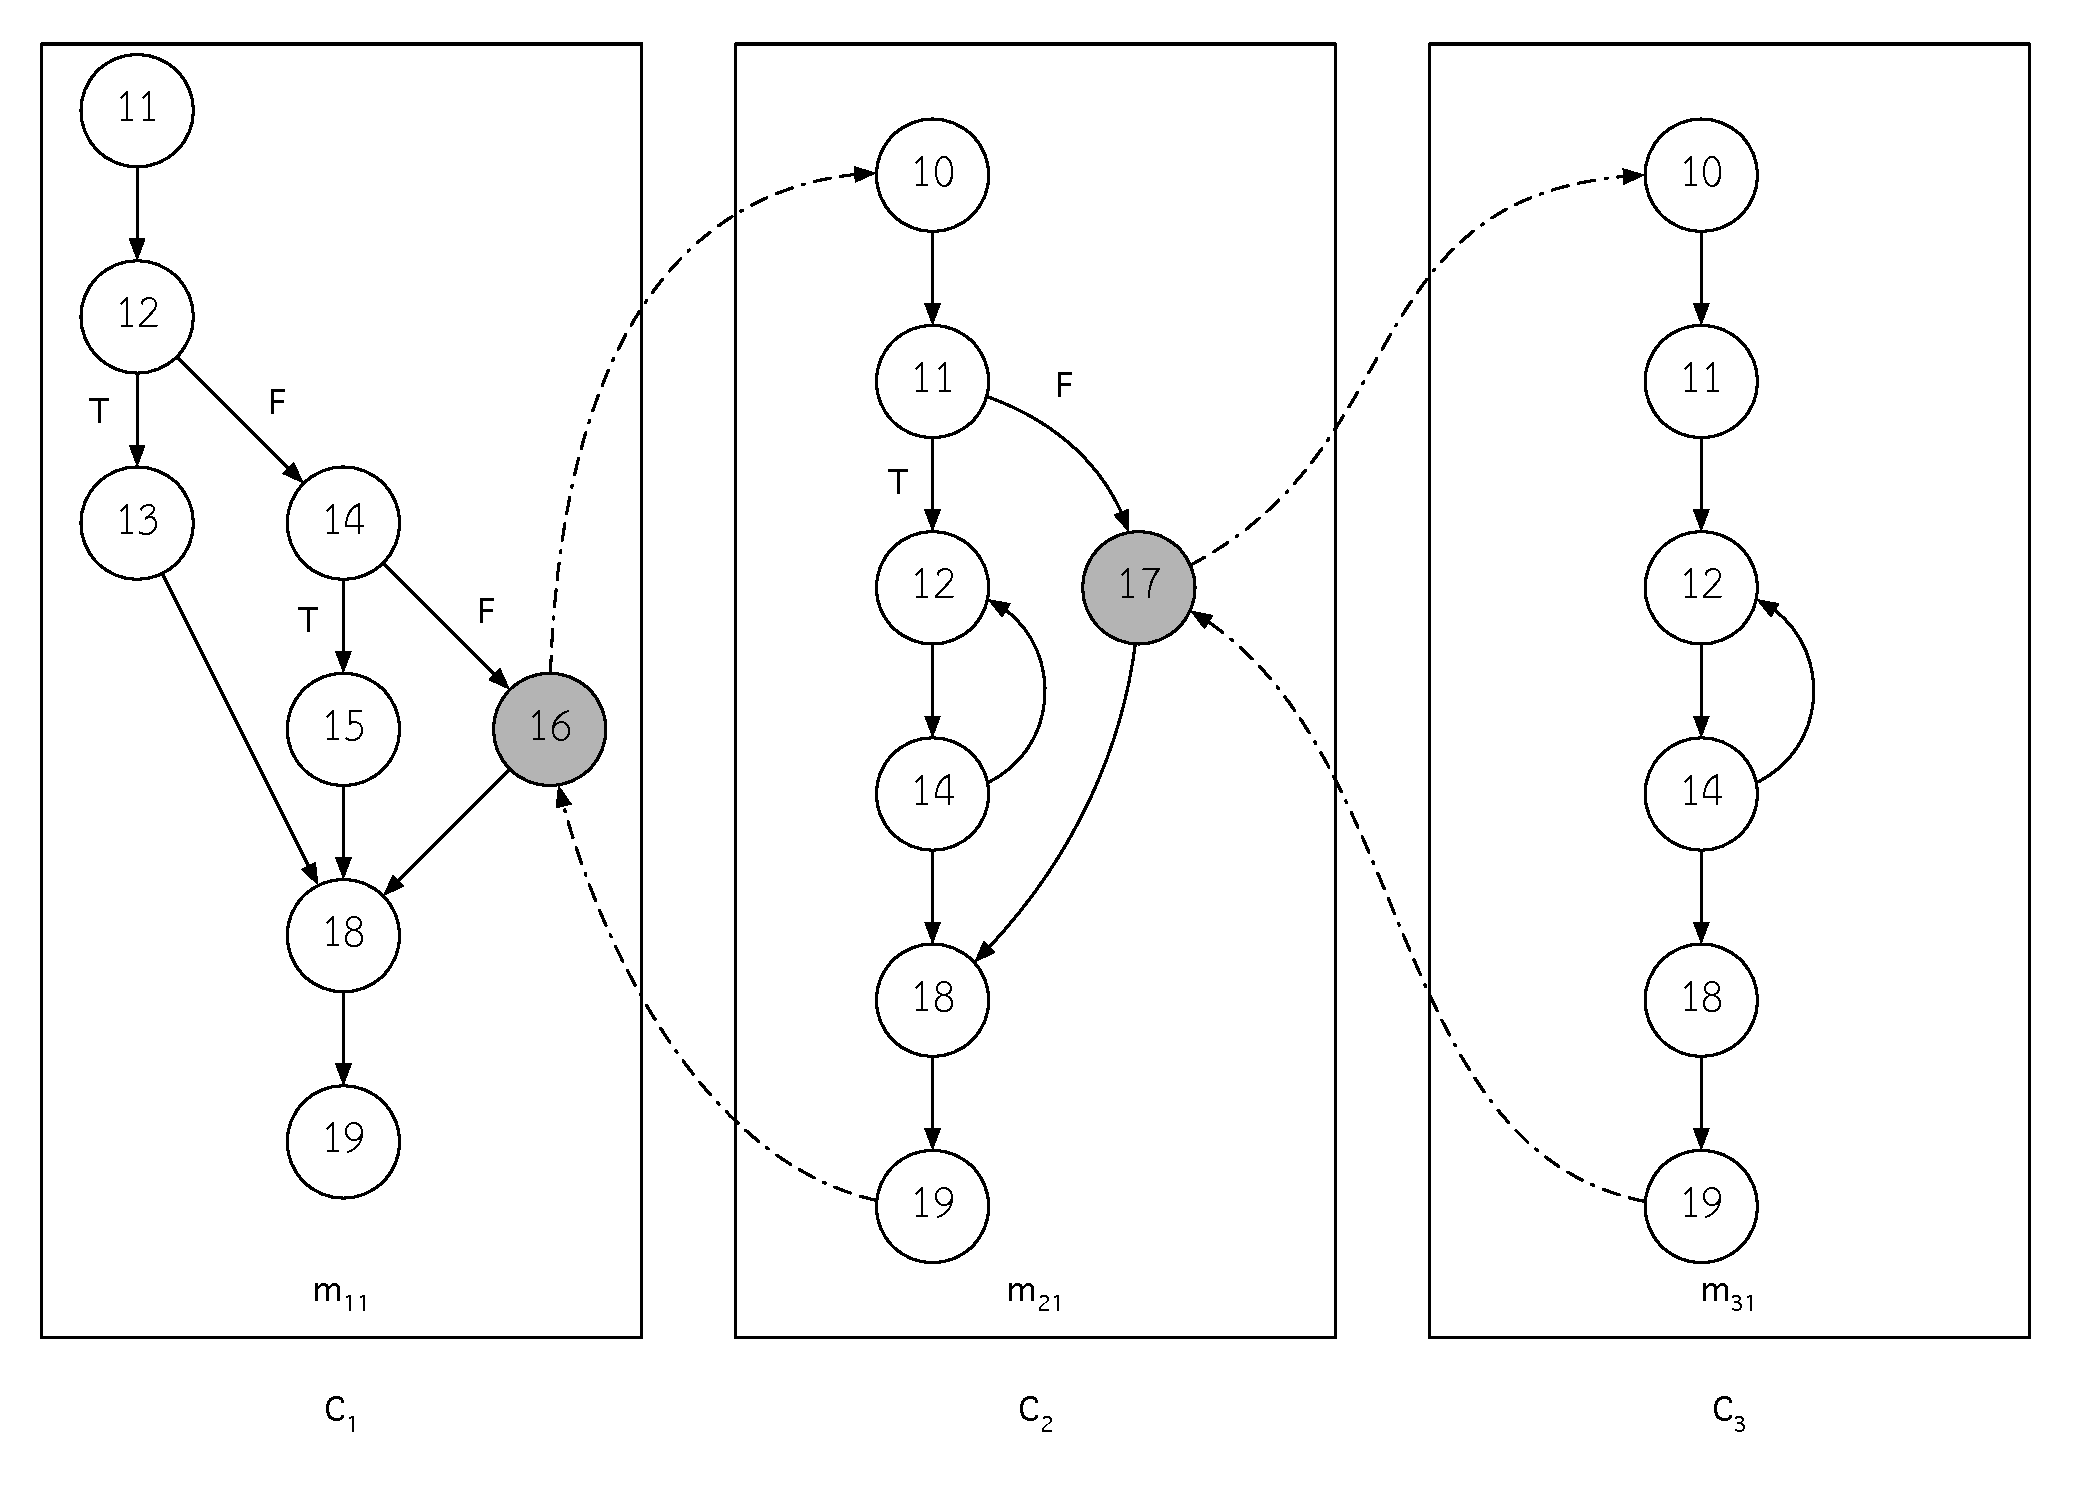
\includegraphics[width=\linewidth]{figures/Calling-statements-of-Classes}
\caption{Calling Statement between Method $m_{11}$ of $C_1$, Method $m_{11}$ of Class $C_2$, and Method $m_{31}$ of Class $C_3$}
\label{fig:callingStatement}
\end{figure}

\subsubsection{Signature Analysis Methods}
This process is performed in order to guide an input domain for random input process 
by signature analysis method, calling and called methods and test path that are transferred 
from the previous process, including the predicate nodes that are found on the test path \cite{Ma2016}. 
For example, a selected path (\figref{fig:callingStatement}) has 3 predicate nodes i.e. 
node $12$, node $14$ of method $m_{11}$, and node $11$ of method $m_{21}$. The random input data 
are guided by conditions found in predicate node.  Thus, input data should conform 
to each predicate node and each predication node must be in line with the conditions provided in 
\figref{fig:conditionsPredicate}

\begin{figure}[ht!]
    \centering
    \makebox[0.7\linewidth][l]{$m_{11}:12~studentScore~>~80$} \par
    \makebox[0.7\linewidth][l]{$m_{11}:14~studentScore~>~50$} \par
    \makebox[0.7\linewidth][l]{$m_{21}:11~true~>~hasQuizScore$}
    \caption{Conditions in Predicate Nodes}
    \label{fig:conditionsPredicate}
\end{figure}
\begin{figure}[ht!]
    \centering
    \makebox[\linewidth][l]{$m_{11}(String\,studentID,\,float\,studentScore)\,:\,String$} \par
    \makebox[\linewidth][l]{$m_{21}(String\,studentID)\,:\,float$} \par
    \makebox[\linewidth][l]{$m_{31}(String\,studentID)\,:\,float$}
    \caption{Method Signatures of $m_{11}$, $m_{21}$, and $m_{31}$}
    \label{fig:methodSignature}
\end{figure}

This is where the test data generation has considered each predicate node provided above. 
Test data should be generated to conform with predicated found in node $m_{11}:12$, 
$m_{11}:14$ and $m_{21}:11$ in order to activate the test case.

With the signature method $m_{11}$, $m_{21}$ and $m_{31}$ as given in \figref{fig:methodSignature}, 
when the test data has considered each predicate above, it is to say that, there is only $studentScore$ 
that we have to consider and ignore for $hasQuizScore$. Because $hasQuizScore$ does not exists in 
method signature. Finally, studentScore should conform predicate node must be lower than 
or equal to $80$ and $50$.


\subsubsection{Random Input Data}
Previously, random data has already randomized the value, but the method could have been more 
than one parameter. That is, each parameter of the method has to be considered. For the parameter 
found in the predicate nodes, it already has a guiding value from the previous process. 
On the other hand, parameters that are not found in the predicate nodes must be randomized 
by using constant value gathered from the constant collection process \cite{Ma2016}

\subsubsection{Test Case Generation}
For this process, test path should be converted to a set of test cases. Test case generation 
must conform to the steps of object creation that can be found in the test path, 
including of the test data formed in the previous process.

\subsection{Expected Output Adjustment}
At this process, test cases are generated; however, they are not actually executed, 
because our approach has gathered only the static data and regardless the behavior method 
such as methods of returning values or input values that do not appear on the test paths. 
The software tester must adjust these values to satisfy the test paths, altogether 
with considering the behavior method.

\subsection{Software Testing Execution}
After expected output adjusted, the software tester has achieved to adjust expected outputs 
of the test cases, the test case must be executed with the instrumented source code 
retrieved from the source code instrumentation process in the local repository. During 
the execution process of the test, we should collect instrumentation messages 
that are displayed when the test cases traverse through nodes of test path.

\subsection{Result Comparison to Graph}
In order to verify a generated test case, we should create a traversing path from 
the instrumentation message that is collected from the previous process and display 
the execution result to the software tester.


% needed in second column of first page if using \IAENGpubid
%\IAENGpubidadjcol

\subsubsection{Subsubsection Heading Here}
Subsubsection text here.

Number equations consecutively with equation numbers in parentheses
flush with the right margin, as in (1). First use the equation
editor to create the equation. Then select the "Equation" markup
style. Press the tab key and write the equation number in
parentheses. To make your equations more compact, you may use the
solidus ( / ), the exp function, or appropriate exponents. Use
parentheses to avoid ambiguities in denominators.


% >>>>>>>>>>>>>>>>>>>> Add an equation <<<<<<<<<<<<<<<<<<<<<<<<<<<<<<<<<<

Equation numbers are automatically generated.  Label allows easy
referencing throughout the paper

\begin{equation}
{\bf X}[k+1]=A{\bf X}[k]+B{\bf u}[k] \label{stateSpaceForm1}
\end{equation}

% >>>>>>>>>>>>>>>>>>> Add an unnumbered equation <<<<<<<<<<<<<<<<<<<<<<<<

You can also add an unnumbered equation as follows

$$
\theta_c[k+1]=\theta_c[k]+Tu_p[k]
$$


The contents of IAENG journals and proceedings books are
peer-reviewed and archival. The journals and proceedings series
publish scholarly articles of archival value as well as tutorial
expositions and critical reviews of classical subjects and topics of
current interest. Authors should consider the following points:

1) Technical papers submitted for publication must advance the state
of knowledge and must cite relevant prior work.

2)  The length of a submitted paper should be commensurate with the
importance, or appropriate to the complexity, of the work. For
example, an obvious extension of previously published work might not
be appropriate for publication or might be adequately treated in
just a few pages.

3) Authors must convince both peer reviewers and the editors of the
scientific and technical merit of a paper; the standards of proof
are higher when extraordinary or unexpected results are reported.

4) Because replication is required for scientific progress, papers
submitted for publication must provide sufficient information to
allow readers to perform similar experiments or calculations and use
the reported results. Although not everything need be disclosed, a
paper must contain new, useable, and fully described information.
For example, a specimen's chemical composition need not be reported
if the main purpose of a paper is to introduce a new measurement
technique. Authors should expect to be challenged by reviewers if
the results are not supported by adequate data and critical details.

5)  Papers that describe ongoing work or announce the latest
technical achievement, which are suitable for presentation at a
professional conference, may not be appropriate for publication in a
journal or proceedings book.



% An example of a floating figure using the graphicx package.
% Note that \label must occur AFTER (or within) \caption.
% For figures, \caption should occur after the \includegraphics.
% Note that IAENGtran v1.7 and later has special internal code that
% is designed to preserve the operation of \label within \caption
% even when the captionsoff option is in effect. However, because
% of issues like this, it may be the safest practice to put all your
% \label just after \caption rather than within \caption{}.
%
% Reminder: the "draftcls" or "draftclsnofoot", not "draft", class
% option should be used if it is desired that the figures are to be
% displayed while in draft mode.
%
%\begin{figure}[!t]
%\centering
%\includegraphics[width=2.5in]{myfigure}
% where an .eps filename suffix will be assumed under latex,
% and a .pdf suffix will be assumed for pdflatex; or what has been declared
% via \DeclareGraphicsExtensions.
%\caption{Simulation Results}
%\label{fig_sim}
%\end{figure}

\begin{figure}[!t]
\centering
\caption{A Simple Neural Network Structure}
\label{fig_nn}
\end{figure}


Figure axis labels are often a source of confusion. Use words rather
than symbols. As an example, write the quantity "Magnetization," or
"Magnetization M," not just "M." Put units in parentheses. Do not
label axes only with units.

Large figures and tables may span both columns. Place figure
captions below the figures; place table titles above the tables. If
your figure has two parts, include the labels "(a)" and "(b)" as
part of the artwork. Please verify that the figures and tables you
mention in the text actually exist.


% Note that IAENG typically puts floats only at the top, even when this
% results in a large percentage of a column being occupied by floats.


% An example of a double column floating figure using two subfigures.
% (The subfig.sty package must be loaded for this to work.)
% The subfigure \label commands are set within each subfloat command, the
% \label for the overall figure must come after \caption.
% \hfil must be used as a separator to get equal spacing.
% The subfigure.sty package works much the same way, except \subfigure is
% used instead of \subfloat.
%
%\begin{figure*}[!t]
%\centerline{\subfloat[Case I]\includegraphics[width=2.5in]{subfigcase1}%
%\label{fig_first_case}}
%\hfil
%\subfloat[Case II]{\includegraphics[width=2.5in]{subfigcase2}%
%\label{fig_second_case}}}
%\caption{Simulation results}
%\label{fig_sim}
%\end{figure*}
%
% Note that often IAENG papers with subfigures do not employ subfigure
% captions (using the optional argument to \subfloat), but instead will
% reference/describe all of them (a), (b), etc., within the main caption.


% An example of a floating table. Note that, for IAENG style tables, the
% \caption command should come BEFORE the table. Table text will default to
% \footnotesize as IAENG normally uses this smaller font for tables.
% The \label must come after \caption as always.
%
%\begin{table}[!t]
%% increase table row spacing, adjust to taste
%\renewcommand{\arraystretch}{1.3}
% if using array.sty, it might be a good idea to tweak the value of
% \extrarowheight as needed to properly center the text within the cells
%\caption{An Example of a Table}
%\label{table_example}
%\centering
%% Some packages, such as MDW tools, offer better commands for making tables
%% than the plain LaTeX2e tabular which is used here.
%\begin{tabular}{|c||c||c|}
%\hline
%One & Two & Five\\
%\hline
%Two & Four & Ten\\
%\hline
%\end{tabular}
%\end{table}

\begin{table}[!t]
\renewcommand{\arraystretch}{1.3}
\caption{An Example of a Table} \label{table_example}
\centering
\begin{tabular}{|c||c||c|}
\hline
One & Two & Five\\
\hline
Two & Four & Ten\\
\hline
\end{tabular}
\end{table}


% Note that IAENG does not put floats in the very first column - or typically
% anywhere on the first page for that matter. Also, in-text middle ("here")
% positioning is not used. Most IAENG journals use top floats exclusively.
% Note that, LaTeX2e, unlike IAENG journals, places footnotes above bottom
% floats. This can be corrected via the \fnbelowfloat command of the
% stfloats package.



\section{Conclusion}
The conclusion goes here.

A conclusion section is not compulsory. Although a conclusion may
review the main points of the paper, do not replicate the abstract
as the conclusion. A conclusion might elaborate on the importance of
the work or suggest applications and extensions \cite{IJCS, EL,
IJAM, WCECS, WCE, IMECS}.




% if have a single appendix:
%\appendix[Proof of the Zonklar Equations]
% or
%\appendix  % for no appendix heading
% do not use \section anymore after \appendix, only \section*
% is possibly needed

% use appendices with more than one appendix
% then use \section to start each appendix
% you must declare a \section before using any
% \subsection or using \label (\appendices by itself
% starts a section numbered zero.)
%


\appendices
\section{Proof of the First Zonklar Equation}
Appendix one text goes here.

% you can choose not to have a title for an appendix
% if you want by leaving the argument blank
\section{}
Appendix two text goes here.


% use section* for acknowledgement
\section*{Acknowledgment}


The authors would like to thank...

The preferred spelling of the word "acknowledgment" in American
English is without an "e" after the "g." Use the singular heading
even if you have many acknowledgments. Avoid expressions such as
"One of us (S.B.A.) would like to thank ... ." Instead, write "F. A.
Author thanks ... ." Sponsor and financial support acknowledgments
are placed in the unnumbered footnote on the first page, not here.


% Can use something like this to put references on a page
% by themselves when using endfloat and the captionsoff option.
\ifCLASSOPTIONcaptionsoff
  \newpage
\fi



% trigger a \newpage just before the given reference
% number - used to balance the columns on the last page
% adjust value as needed - may need to be readjusted if
% the document is modified later
%\IAENGtriggeratref{8}
% The "triggered" command can be changed if desired:
%\IAENGtriggercmd{\enlargethispage{-5in}}

% references section

% can use a bibliography generated by BibTeX as a .bbl file
% BibTeX documentation can be easily obtained at:
% http://www.ctan.org/tex-archive/biblio/bibtex/contrib/doc/
% The IAENGtran BibTeX style support page is at:
% http://www.michaelshell.org/tex/IAENGtran/bibtex/
%\bibliographystyle{IAENGtran}
% argument is your BibTeX string definitions and bibliography database(s)
%\bibliography{IAENGabrv,../bib/paper}
%
% <OR> manually copy in the resultant .bbl file
% set second argument of \begin to the number of references
% (used to reserve space for the reference number labels box)
% \begin{thebibliography}{1}

% \bibitem{IJCS}
% N.~Meghanathan and G.~W. Skelton, ``Risk Notification Message
% Dissemination Protocol for Energy Efficient Broadcast in Vehicular
% Ad hoc Networks,'' {\it IAENG International Journal of Computer
% Science}, vol. 37, no. 1, pp. 1-10, Jul. 2010.

% \end{thebibliography}


% >>>>>>>>>>>>>>>>>>>>>> Bibliography <<<<<<<<<<<<<<<<<<<<<<<<<<<<<<<<<<<<<

\bibliographystyle{BibTeXtran}   % (uses file "BibTeXtran.bst")
\bibliography{BibTeXrefs}       % (expects the reference in the file "BibTeXrefs.bib")


\end{document}
